\documentclass[english]{DESCARWINreport}

\usepackage{amsmath}
\usepackage{amsfonts}
\usepackage{color}
\usepackage{algorithm}
\usepackage[noend]{algorithmic}
%\usepackage{algorithmic}
\usepackage{subfigure}
\usepackage{hyperref}
\hypersetup{colorlinks=true,linkcolor=black}
\usepackage{lscape}
\title{DESCARWIN\\\bigskip {\em \LARGE The Marriage of Descartes and Darwin}\\\vspace{8cm} 
{\LARGE D3.3\\
Multi-Objective Experimentations}}
%ANR-09-COSI-002
%\author{Pierre Savéant and Johann Dréo}
\date{\today}
\laboratory{TRT - INRIA - ONERA}
\docref{62 441 217-306}
\revision{-}

\setlength{\parindent}{0cm}
\setlength{\parskip}{2ex plus 0.5ex minus 0.2ex}

\newcounter{hyp}
\setcounter{hyp}{1}
\newcommand{\hyp}{H\thehyp\stepcounter{hyp}}
\newcounter{defi}
\setcounter{defi}{1}
\newcommand{\defi}{D\thedefi\stepcounter{defi}}
\newcounter{con}
\setcounter{con}{1}
\newcommand{\con}{C\thecon\stepcounter{con}}

% Pour réduire globalement l'espace entre les items d'une liste
% on peut également utiliser le bout de code suivant de M. Wooding
% Les paramètres utilisés pour définir cette mise en page
% sont les suivants :
% \topsep espace vertical supplémentaire (ajoute à \parskip)
% 	inséré entre le texte précédant la liste et le 1er objet
% 	de la liste
% \partosep espace vertical supplémentaire inséré devant la liste
% 	si celle-ci est précédée d'une ligne blanche
% \itemsep espace vertical supplémentaire (ajouté à \parsep)
% 	inséré entre les éléments d'une liste.

%%%% debut macro %%%%
\makeatletter
\toks@\expandafter{\@listI}
% \edef\@listI{\the\toks@\setlength{\parsep}{0pt}}
% \edef\@listI{\the\toks@\setlength{\topsep}{0pt}}
\makeatother
%%%% fin macro %%%%

\usepackage[final]{pdfpages}

\hoffset -2cm
\textwidth 15cm


\def\dae{{\em Divide-and-Evolve}}
\def\DAE{{\sc DaE}}
\def\DAEX{{\sc DaE$_{\text{X}}$}}
%\def\DAEYAHSP{{\sc DaE$_{\text{YAHSP}}$}}
\newcommand{\DAEYAHSP}{{\sc DaE$_{\text{YAHSP}}$}}
\def\PARADISEO{{\sc ParadisEO-MOEO}}
\def\YAHSP{{\sc YAHSP}}
\def\CPT{{\sc CPT}}
\def\modae{{\em Multi-Objective Divide-and-Evolve}}
\def\MODAE{{\sc MO-DaE}}
\def\ZENO{{\sc Zeno}}
\def\MULTIZENO{{\sc MultiZeno}}
\def\PARAMILS{{\sc ParamILS}}


\begin{document}

\maketitle

%\cleardoublepage

\begin{revisions}
\begin{revtable}
\dates{May 7., 2013}{}{}{}{}
\writers{Mostepha Khouadjia\\Pierre Savéant\\Marc Schoenauer\\Vincent Vidal}{}{}{}
\approvers{P. Sav\'eant}{}{}{}
\end{revtable}
\begin{revisionlabels}
\revlabel{initial version}
\revlabel{}
\end{revisionlabels}
\end{revisions}

%\begin{figure}[htbp]
%\vspace{-0.5cm}
%\centering
%\includegraphics[width=0.25\textwidth]{Salon_du_Bourget_20090619_114_GroundSearch_1000km.jpg}
%\end{figure}

\begin{abstract}
The object of this document is to provide results of the experimentation campaign regarding the original multi-objective approach to AI planning developed in the DESCARWIN project. As far as we know, \DAE\ is the only existing multi-objective, Pareto-based approach of AI Planning. Chapter 5 will compare to the only work that we know of that tackles the same problem (multi-objective AI planning), based on the so-called metric-sensitive planner, an approach that is very similar to the well-known aggregation approach, and a priori suffers similar defects. 

This deliverable is made of 3 chapters, corresponding to 3 publications describing the different steps of the experimental campaign that validates the proposed approach. Each chapter starts with an extended abstract that introduces the context of the work, followed by a copy of the published paper.

\begin{itemize}
 \item The first validation was performed on the original {\tt Zeno} benchmark suite, as described in Deliverable 3.1. The benchmark is first described in detail, and the experimental parts compare several multi-objective evolutionary engines in several instances of this benchmark. And the winner is (on the Zeno testbench at least) \ldots the Indicator-Based Evolutionary Algorithm (IBEA) that uses as indicator the hypervolume. Hence only $IBEA_{Hv}$ has been considered in all following experiments.

This work has been published as: ``Mostepha Redouane Khouadjia, Marc Schoenauer, Vincent Vidal, Johann Dréo and Pierre Savéant, {\em Multi-Objective AI Planning: Evaluating DaEYAHSP on a Tunable Benchmark}. In Robin C. Purshouse, Peter J. Fleming, and Carlos M. Fonseca, Eds, Proc. 7th International Conference on Evolutionary Multi-Criterion Optimization (EMO2013), pp 36-50, LNCS 7811, Springer Verlag, 2013.'' 

\item The second validation compares the Pareto-based approach that was found the best-performing in the previous chapter, i.e. $IBEA_{Hv}$, with the more traditional aggregation-based approach using the single objective version of \DAE. An interesting issue is that of the measure to use within ParamILS, the off-line parameter tuning procedure, for the aggregated approach: the discussion about this issue is reported in Deliverable 2.3, and was surprising enough to be published in the LION'7 conference, and hence will not be detailed in this deliverable. The results presented here all use the hypervolume indicator as a measure of goodness for the tuning of the aggregated single-objective runs. The testbench is, again, the {\tt Zeno} benchmark, and most results demonstrate the superiority of the Pareto-based multi-objective approach compared to the aggregated approach, both in terms of quality of the solution and in terms of speed.

This work has been published as: ``Mostepha Redouane Khouadjia, Marc Schoenauer, Vincent Vidal, Johann Dréo and Pierre Savéant, {\em Multi-Objective AI Planning: Comparing Aggregation and Pareto Approaches}. In Martin Middendorf and Christian Blum, Eds, Proc. 13th European Conference on Evolutionary Computation in Combinatorial Optimisation (EvoCOP2013), pp 202-213, LNCS 7832, Springer Verlag, 2013.''

\item The last series of experiments validates the multi-objective \DAEYAHSP\ approach against the only competitor from the AI Planning community, i.e. the approach using the metric-sensitive planner LPG, one of the state-of-the-art planner in single-objective setting, that can however directly handle aggregated objectives. The comparative experiments here involve not only the {\tt Zeno} test-bench, but also the other domains and instances proposed in Deliverable 3.1 based on the multi-objectivizations of some IPC7 (single-objective) domains. In most cases, \DAEYAHSP\ is found to outperform the LPG-based approach.

This work has been accepted at IJCAI 2013 conference, August 2013, as ``Mostepha Redouane Khouadjia, Marc Schoenauer, Vincent Vidal, Johann Dréo and Pierre Savéant, {\em Pareto-Based Multiobjective AI Planning}. In Proc. 23rd International Joint Conference on Artificial Intelligence (IJCAI 2013), 2013.''
\end{itemize}

It is worth mentioning here that all experiments that are described in this deliverable include an intensive parameter tuning phase before any result is reported. The whole of WP2 was devoted in DESCARWIN to the issue of parameter tuning. More specifically, the detailed procedure that was used in all experiments described here are based on the ParamILS framework, as described in more details in Deliverable 2.3.


\end{abstract}

%\begin{figure}[htbp]
%\centering
%\includegraphics[width=0.70\textwidth]{../Images/Salon_du_Bourget_20090619_114_GroundSearch_1000km.jpg}
%\end{figure}

\tableofcontents

\newpage

\chapter{Evaluating \DAEYAHSP\ on a Tunable Benchmark}

After the seminal paper in EvoCOP 2006 by Schoenauer, Savéant and Vidal [7]\footnote{The references are those in the published paper that follows.}, that gave a very simple proof-of-principle of the multi-objectivization of \DAE\, the topic had been left untouched until this publication in the EMO 2013 conference. Two reasons at last explain that.
\begin{itemize}
 \item There was no real interest in the AI Planning community for multi-objective problems: though a multi-objective track had been organized during IPC5 (2006) and IPC6 (2008), it was canceled in the latter, and abandoned for IPC7 (2011), even though it was targeted at aggregation approaches. Hence we felt that our proposition for a Pareto-based multi-objective AI planner would probably be hard for that community to accept.
 \item The results obtained by this preliminary version of \MODAE\ were in fact rather poor. One reason was that the embedded planner was \CPT\ and not \YAHSP\ -- and it has been demonstrated since then that, in the single-objective context, the latter allows far better results than the former; Another reason was that \CPT\ was only able to optimize the makespan, even though it could compute the cost along a given plan, whereas \YAHSP\ can today optimize either objective (see the discussion in Section 6.2 in the following paper).
\end{itemize}

Things have now changed, both in the community, with the recent work for instance of Sroka and Long (see exact reference in the paper in Chapter 4), and around \DAE\, with the use of the recent version of \YAHSP. This work, published in EMO'2013 (April 2013 in Sheffield), can hence be considered as the first actual validation of the \MODAE\ approach, while \MODAE\ can be considered as the first Pareto-based multi-objective AI planner.

In this first paper, we rapidly recall the basics of \DAE\ in Section 2 -- the single-objective version, though the representation and the variation operators are of course independent of the number of objectives: this flexibility is one of the great strengths of Evolutionary Algorithms, you ``only'' need to change the selection procedure to turn a single-objective EA into a multi-objective one.

But many possible multi-objective schemes have been published, and reported efficient. Together with the baseline of \MODAE\, Section 3 introduces what can be seen as the 4 most popular and efficient ones (see reference in the corresponding Section of the paper), NSGA-II, SPEA2, and two recent Indicator-based algorithms, one using the Hypervolume indicator, the other based on the additive Epsilon indicator. Note that the EvoCOP paper only used NSGA-II.

Importantly, Section 4 details the original benchmark that we propose here, extending a benchmark proposed in the seminal EvoCOP paper in 2006: the \MULTIZENO\ benchmark, based on the famous \ZENO\ benchmark present in all IPCs. In particular here, we detail how the basic instance proposed in 2006 can be complexified, resulting in a full benchmark suite for which the exact Pareto front is known (at least for small instances), and where its shape can be modified by modifying some durations and costs -- though at the moment, we have proceeded by trials-and-errors to obtain 3 different fronts, linear, convex and ``concave'' (i.e., with some concave parts), as can be seen on Figure 2 of the following paper. Note that further trials have led to a much ``less convex'' Pareto front, as can be seen on Figure 2 of the paper in Chapter 3.

Section 5 introduces the experiments, that are presented and discussed in Section 6, using both the evolution of the hypervolume with the number of evaluations, and the proportion of runs that reach each of the points on the Pareto front, as the fronts are all know exactly here. Some of the presented results also include the complete 'fronts' returned by the runs, as sometimes the front is not reached, but the difference between the result and the front is rather tiny. In any case, it is important to remember that all algorithms had been tuned using \PARAMILS, based on the hypervolume indicator of the final population for a measure of the algorithm performance, and all comparisons were validated using statistical tests (here, the Wilcoxon signed rank test, see Table 1 for instance).

The main conclusion of the paper is that the best performing scheme is the $IBEA_{H-}$ scheme, the indicator-based algorithms using the hypervolume as indicator. Further work will only involve this algorithm from thereon. 


\newpage
\hoffset 0cm
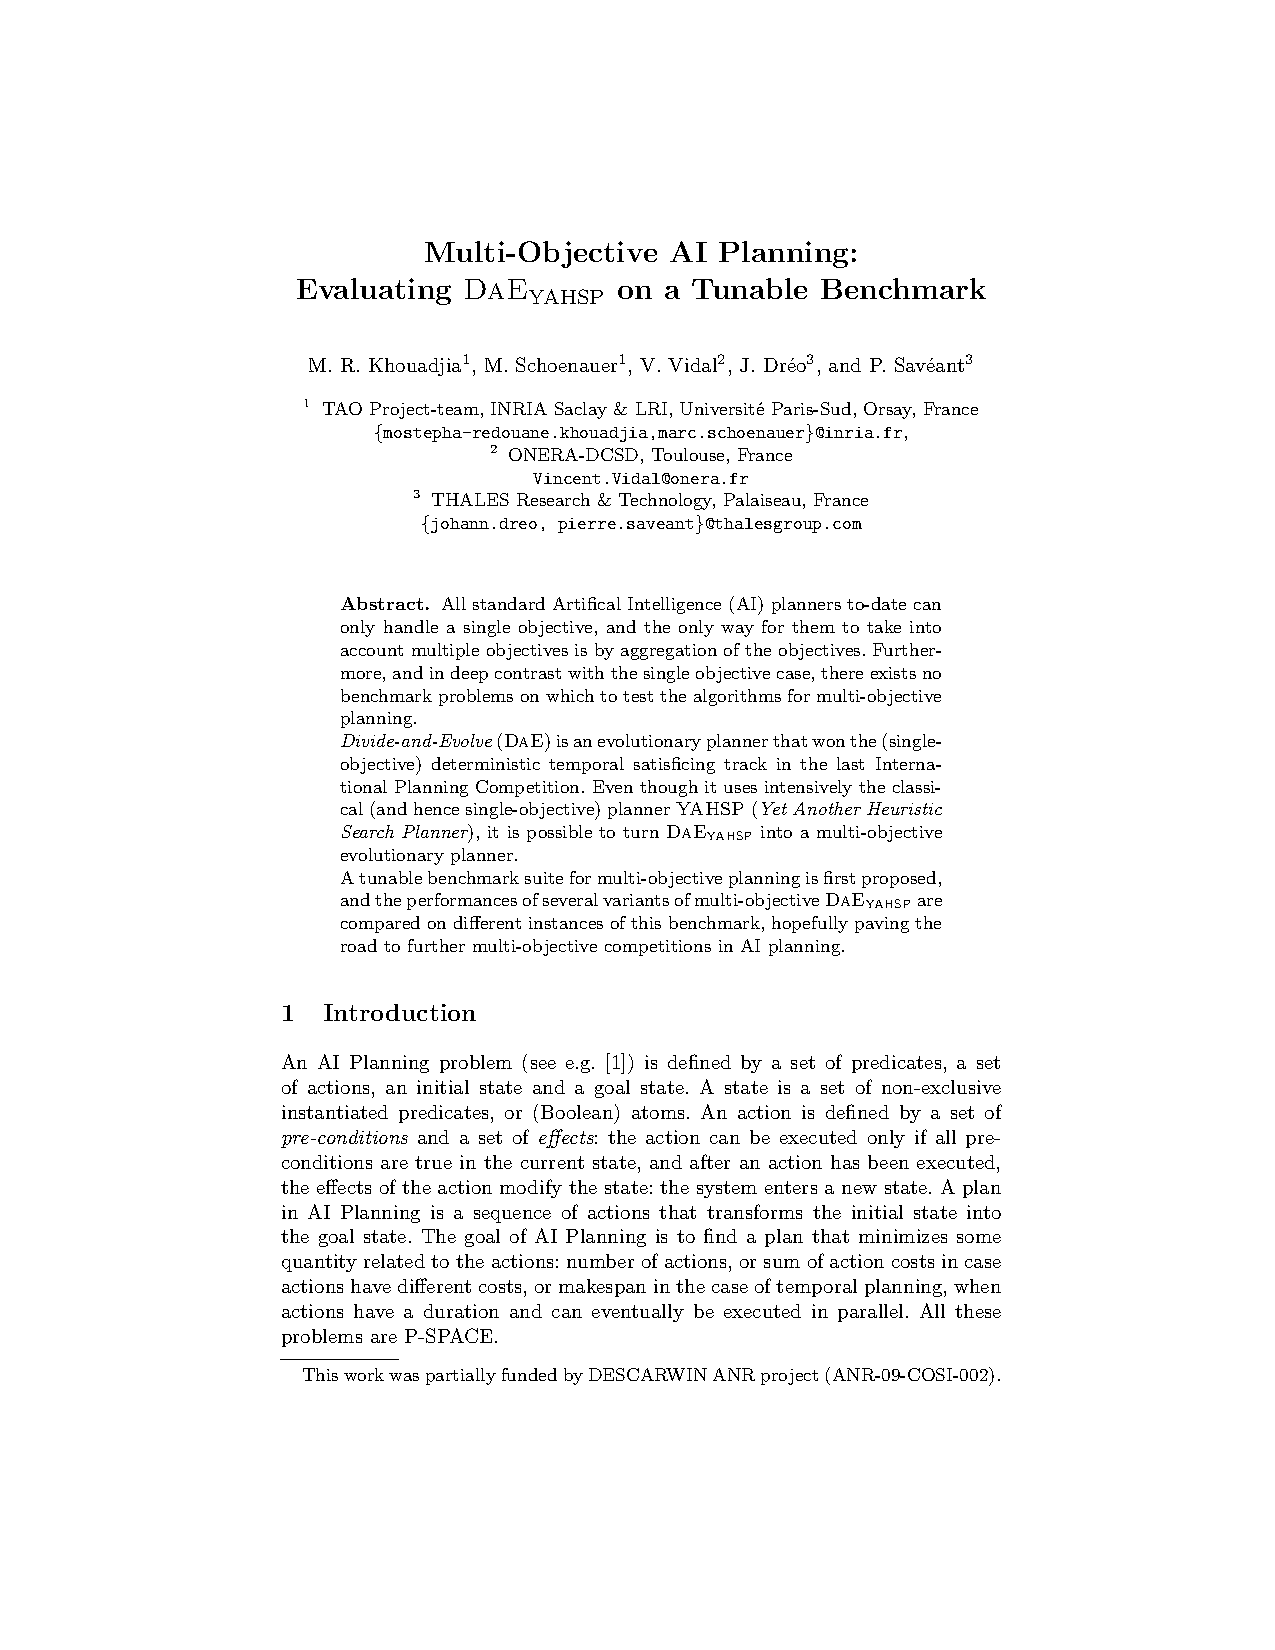
\includepdf[height=32cm,pages=-,offset=0cm -4cm]{emo2012.pdf}
\newpage
\hoffset -2cm

\chapter{Comparing Aggregation and Pareto Approaches}

One of the main arguments to justify the use of Pareto-based approaches for multi-objective optimization in general is that they are more efficient than the naive aggregation approach, that can be implemented in no time using any single-objective optimizer. It was hence mandatory to check that it was the case too in the \DAE\ framework. The following work was hence dedicated to a thorough comparison between \MODAE, as proposed in the previous Chapter, and the aggregated approach based on \DAE\ itself (single-objective version).

The basic idea of the aggregated approach is to launch several runs optimizing weighted sums of the objectives with different weights. The so-called $\alpha$-run thus optimizes $\alpha F_1 + (1-\alpha) F_2$, $F_1$ and $F_2$ being the two objectives, and $\alpha$ taking values in $[0, 1]$. Several values of $\alpha$ are chosen (here, \{0, 0.1, 0.3, 0.5, 0.7, 0.9, and 1\}), and the results of those 7 runs are merged together, retaining the non-dominated individuals from this merged population as the result of the aggregated run.

As in all our work, parameter tuning plays an important role here - and each of the $\alpha$-runs was separately tuned using ParamILS (Table 1 gives the list of the parameters that have been taken into account and optimized by ParamILS). Two important issues should be highlighted here regarding this parameter setting phase.
\begin{itemize}
\item Among these parameters, are the weights that govern the choice of \YAHSP\ strategy with respect to both objectives. As already mentioned, \YAHSP\ can optimize either objective, but not a weighted sum of the objectives. It had already been pointed out in previous Chapter on the hitting plots of the Pareto fronts that systematically using one strategy (i.e., optimizing only one objective) resulted in increasing the probability to discover the points on the corresponding part of the Pareto front, and this is why the choice of \YAHSP\ was randomized, governed by some user-defined weights. In this Chapter, the reverse conclusion was drawn from the automatic parameter tuning strategy: in all runs of ParamILS on \MODAE, the weights that govern the choice of \YAHSP\ strategy were found to be equal in the optimal setting: it is mandatory to avoid any bias in that respect to increase the performance of the algorithm.
\item Not mentioned here because of tight space constraints, the metric that was used to tune each of the $\alpha$-runs was in itself a topic worth investigating, and this has been reported in Deliverable D2.3, Chapter 5 and published in the LION'7 conference in January 2013. The naive approach would be to use for ParamILS metric the same one that is optimized by the algorithm - the best fitness obtained in the final population of a run. However, though each $\alpha$-run is unaware of the global goal here (minimizing the hypervolume of the merged final population of the 7 $\alpha$-runs), it turned out that better results were obtained when the parameters of each of the $\alpha$-runs was tuned using the hypervolume of the final population as a measure of algorithm performance. So all experiments done in this Chapter with the aggregated approach used the parameters given by ParamILS based on the hypervolume of the final population.
\end{itemize}

All experiments presented here were run on the \MULTIZENO\ benchmark suite - basically the \MULTIZENO3, \MULTIZENO6 and \MULTIZENO9 instances, for the 3 shapes of the Pareto front shown in Figure 2 (as mentioned in previous Chapter, the ``concave'' benchmark was here improved compared to the one described there). Another difference with the previous study is that both the {\sc Cost} and the {\tt Risk} problems were considered here, whereas only the {\sc Cost} had been studied previously. Except for the smallest instance \MULTIZENO3, that was too easy in all configurations, it turned out that the {\sc Risk} problems were too difficult, even though the \MODAE\ approach could reach more points on the Pareto front than the aggregated approach.

On the {\sc Cost} problems \MULTIZENO6 and \MULTIZENO9, the \MODAE\ approach is a clear winner of the comparison, even though none identifies the whole Pareto front at every run for \MULTIZENO9. Even if the average hypervolume (over 11 independent runs) of the aggregated approach is slightly better than that of \MODAE, looking at the final populations clearly demonstrates that \MODAE\ is more robust, with its whole population on the Pareto front for \MULTIZENO6, and very close to it for \MULTIZENO9, while the aggregated approach displayed a much wider dispersion. 
Similar conclusion could also be drawn from the results on the different instances of the benchmarks, with different Pareto shapes. 

A final word regarding the cost of these algorithms: for the sake of comparison, all $\alpha$-runs were tuned anew for each value of $\alpha$, but the cost of the parameter setting phase was not counted here, only the number of function evaluations of the tuned algorithms was taken into account. Hence the actual cost of the aggregated approach, including the cost of parameter setting, would in fact be much higher than that of the Pareto-based \MODAE. And a few trials with less values of $\alpha$ showed, as expected, a decrease in quality of the results.

The conclusion of this series of experiments is that indeed, the Pareto-based approach outperforms the aggregated approach solely based on the single-objective \DAE.

\newpage
\hoffset 0cm
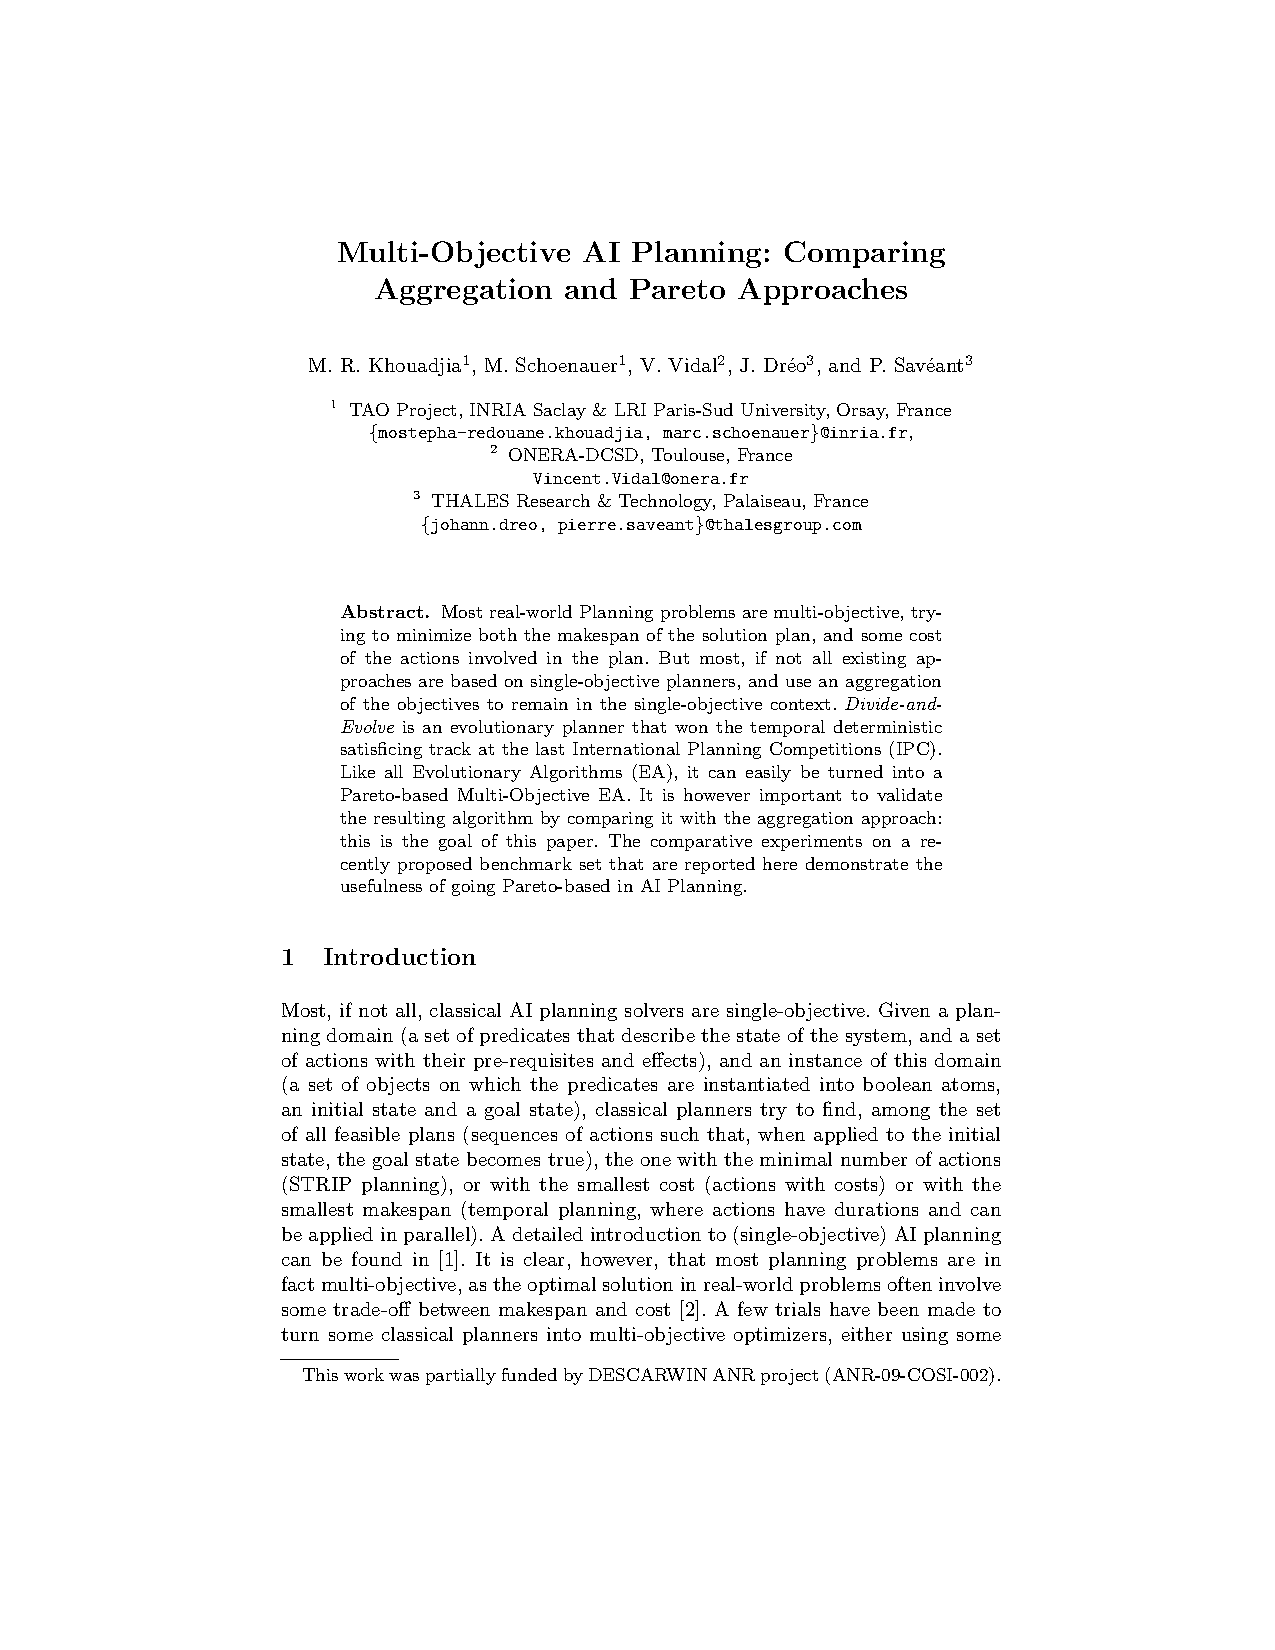
\includepdf[height=32cm,pages=-,offset=0cm -4cm]{evocop2012.pdf}
\newpage
\hoffset -2cm

\chapter{Comparing Metric-Sensitive and Pareto Approaches}

Previous Chapter has compared the Pareto-based \MODAE\ approach with an aggregated approach, but the aggregated approach was also based on \DAE\ principles. However, in order to be credible within the AI Planning community, we also had to compare the \MODAE\ approach to its only competitor, as far as we can tell, which is based on metric-sensitive planners, and whose champion (and only recently published work up to now) is using LPG [Geverini et al., 2008]\footnote{detailed references in the following publication.}. Metric-sensitive planners are able to actually optimize a weighted sum of the objectives, i.e. to use a weighted sum within the internal mechanisms that guide their search. The use of LPG for multi-objective optimization was published by Sroka and Long [2012a]. 

For the sake of a fair comparison, we obtained the code that had been used by Sroka and Long from the authors (they used Geverini's code as published on his web site, and some scripts to run the different $\alpha$-runs). However, we couldn't run the same benchmarks than the ones they published, because these benchmarks involve numerical fluents, and \YAHSP\ cannot handle numerical fluents at the moment. We hence had to use other benchmarks.

Of course, we used the \MULTIZENO\ benchmark suite, as described in both previous Chapters. But we also used, for the first time, the benchmarks that we had built based on IPC7 domains and instances, as described in Deliverable D3.1, i.e., either merging similar instances in the sequential and temporal tracks, or adding some cost to temporal track domains.

Regarding parameter tuning, a crucial aspect of all experiments in DESCARWIN, the methodology adopted here was slightly different than that of the previous series of experiments presented in Chapters 2 and 3. In those previous works, a full ParamILS optimization of \MODAE\ parameters was run anew for every instance, and for all considered algorithms. Such approach is not realistic in real life, being far too costly (up to 48h for the complete set of instances of \MULTIZENO\ for instance). In these experiments, only one parameter setting was conducted for each domain, on a medium-size instance, and the resulting set of parameters was used for all instances of the domain -- a trade-off between full optimization and computational cost. 

However, no parameter tuning was done, or could be done, for the LPG approach, as only one parameter of LPG is exposed in the publicly available version (it seems that there are some parameters that it could be beneficial to tune, but at the moment they are hidden/hard-coded in the code). Furthermore, this only visible parameter for LPG, tuning the ``locality'' of the search, turned out to be threshold-like: large values resulted in no result at all, while all low values below some threshold all gave very similar results. This parameter was hence set to some low value (LPG working in local mode), and we only checked that the value was low enough for LPG to give some results (though on some instances LPG never gave any result, as can be seen in Section 6 of the published paper).

Because this paper was targeted toward the AI Planning community, as present at IJCAI, the paper had to recall the basic of Evolutionary Multi-objective optimization as well as the ground ideas of \DAE\ and \MODAE. In particular, the paper displays (Figure 4-a) a graphical view of the influence of \YAHSP\ strategy on the evaluation of one single individual. This plot doesn't only reveal the large influence of \YAHSP\ strategy, at least on some instances (few other instances didn't show any difference between strategies), but it also make it very clear that \DAE\ evaluations are very noisy indeed, due to \YAHSP\ stochasticity -- something that we probably had overlooked until now. This suggest some further investigation in that direction, as such feature could be beneficial in an evolutionary setting. 

In order to be as self-sufficient as possible, the paper also needed to introduce the multi-objective benchmarks, as they are not known (unlike IPC single-objective benchmarks). We nevertheless succeeded in demonstrating the advantage of using \MODAE\ in its Pareto-based approach over using even the best available metric-sensitive planner (LPG) with its aggregated approach: this was obvious on the \MULTIZENO\ benchmarks, where even on the rather easy \MULTIZENO6 instance, LPG failed to identify any point close to the Pareto front; This was also clear on most IPC-based instances, with one noticeable exception in the {\tt floortile} domain.

\newpage
\hoffset 0cm
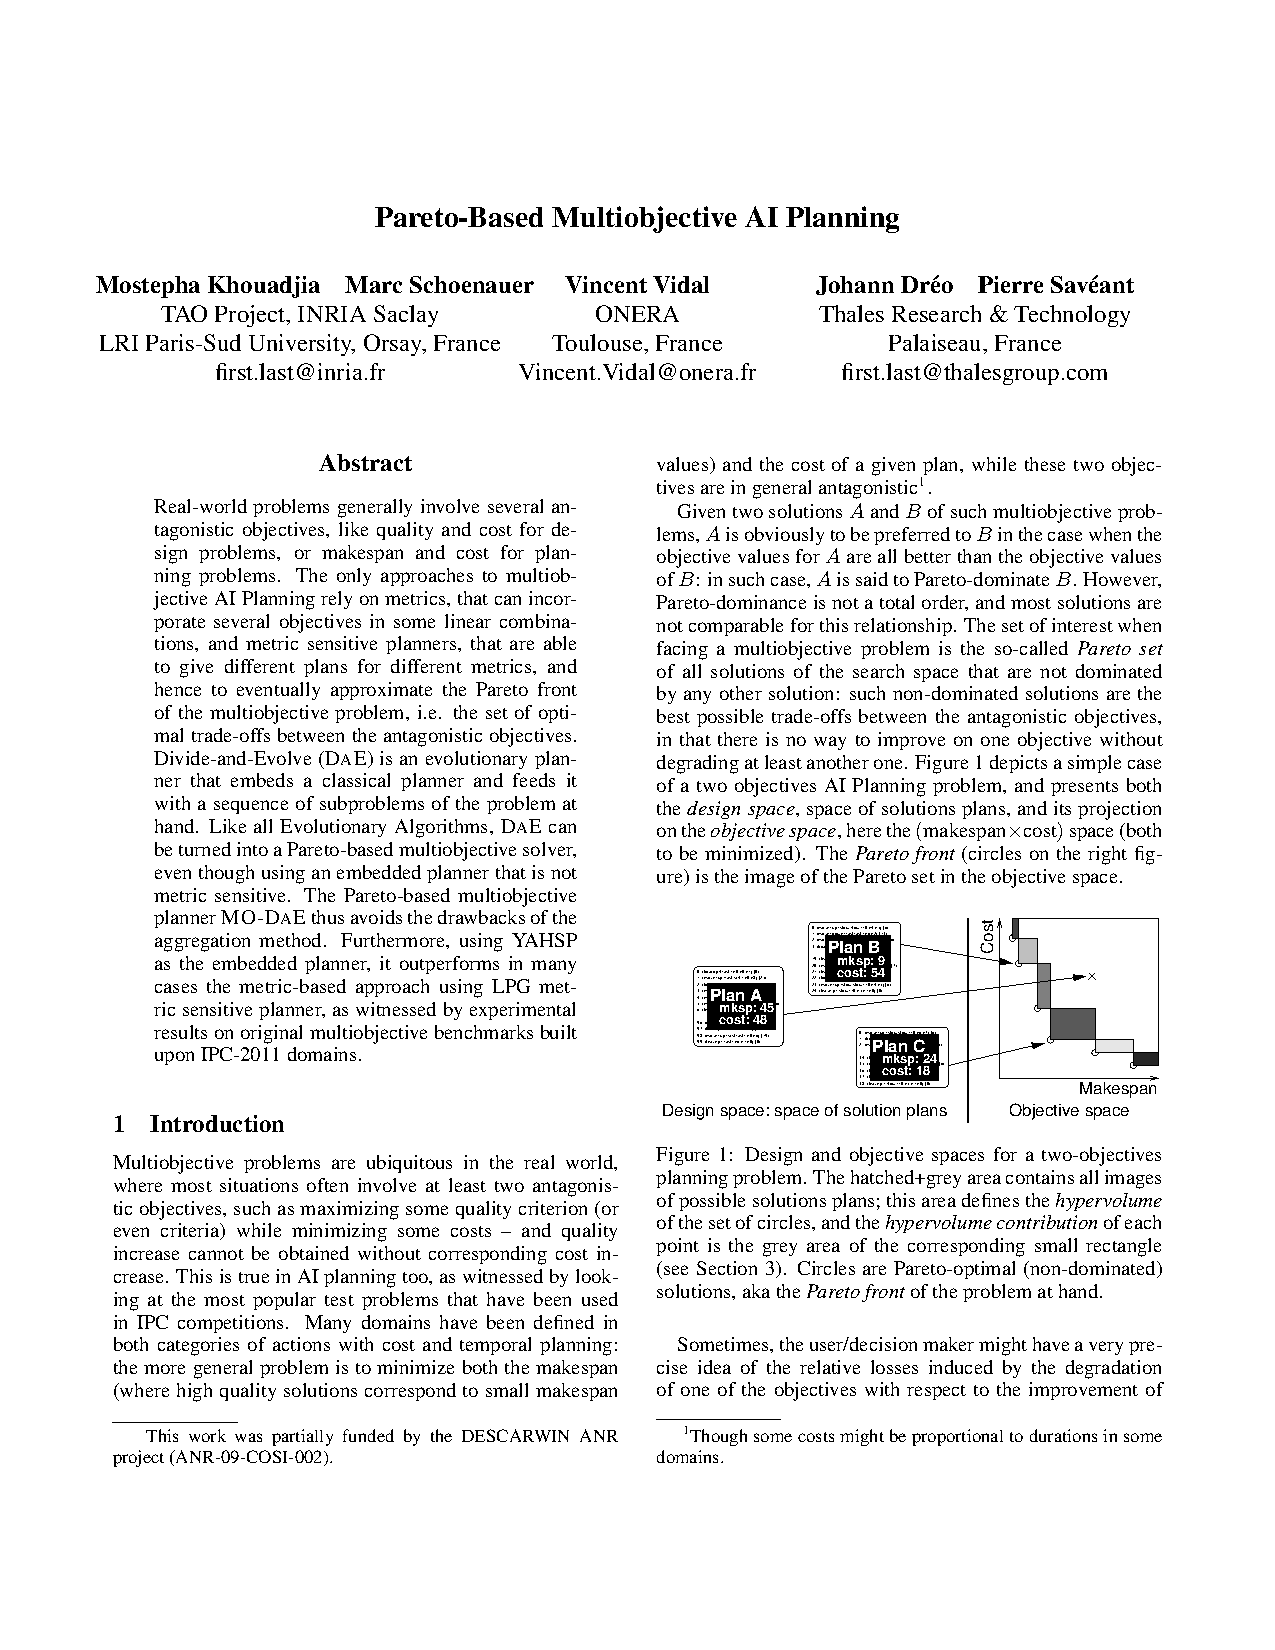
\includepdf[width=22.5cm,height=32cm,pages=-,offset=0cm -4cm]{567.pdf}
\hoffset -2cm

\newpage
\hoffset -2cm

\chapter{Conclusion}

This deliverable somehow witnesses the sum of efforts devoted within the DESCARWIN project to the study of a multi-objective variant of \DAE. The resulting algorithm, \MODAE, is the first Pareto-based approach to multi-objective AI Planning, and we demonstrated its advantages over the classical aggregation approaches, should they use the \DAE\ way or be based on metric-sensitive planners like LPG.

The importance of multi-objective problems in all domains of human activities should not need to be emphasized, even if the AI Planning community seems to only slowly realize it. For instance, there still isn't any multi-objective track in the forthcoming IPC in 2014. However, an ever growing group of people from that community are becoming aware of this field, and we obtained a reasonable success at last ICAPS (Rome, June 2013) when we presented this work to several experts of the field. 

Beyond the first Pareto-based multi-objective AI planner, our contribution to the field also lies in the benchmark suites that we have proposed: from the simple \MULTIZENO\ domain, that can be instantiated into problems of tunable complexity, to different ways to multi-objectivize some well-known IPC domains. 

A lot of work remains to be done. At the algorithmic level, for instance, the parameter that governs \YAHSP\ strategy could be made self-adaptive, at the individual level or at the intermediate problem level; the stochasticity of \YAHSP\ evaluations could be used to improve the fitness of all individuals by some local search (repeated calls to \YAHSP). At the benchmark level, the true Pareto fronts of existing benchmarks should be sought, and in particular it should be possible to find more complex shapes of Pareto fronts. And, of course, a multi-objective track should be (re-)opened in one of the forthcoming IPC.

However, we believe that we have laid the foundations of multi-objective AI Planning in a way that cannot be undone now (unlike the first premature attempt in 2006). And we intend to continue our efforts in that direction.



\end{document}